\begin{flushleft}
Generalmente la legge che descrive un dato fenomeno è di tipo polinomiale con un determinato grado $m$:
\[
y = \sum_{k=0}^{m}(a_k\cdot x^k)
\]
Sapendo che $(x_i,y_i)$ sono misure sperimentali è necessario estrapolare i vettore $a_k$ che meglio approssima il polinomio. Per il calcolo di $a_k$ abbiamo scritto la seguente function:
\lstinputlisting[language=matlab]{cap_4/polBetter.m}
Abbiamo poi testato il suo funzionamento con il seguente script:
\lstinputlisting[language=matlab]{cap_4/es8/es8.m}
Che restituisce in output:
\begin{figure}[H]
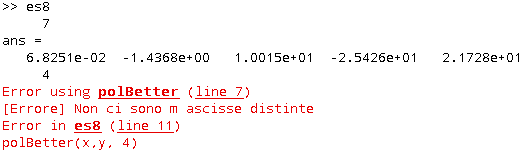
\includegraphics[left, width=400px, height=200px]{cap_4/es8/es48.png}
\end{figure}
Possiamo notare che il secondo insieme di dati sperimentali non ha un numero di ascisse distinte, infatti $4>m+1=5$ non è verificato.
\end{flushleft}